
%\renewcommand{\familydefault}{\sfdefault}
%=============== En−Tete ===============
 
%−−− Insertion de paquetages −−−−
\documentclass[12pt,a4paper]{report}
\usepackage[utf8]{inputenc}
\usepackage{amsmath}
\usepackage{amsfonts}
\usepackage{amssymb}
\usepackage{graphicx}
\usepackage{wrapfig}
\graphicspath{ {./images/} }
\usepackage[rightcaption]{sidecap}
\usepackage{subcaption}

\usepackage[french]{babel}
\usepackage[Bjarne]{fncychap}
\usepackage{fancyhdr}
\usepackage{float}
\usepackage{epsfig}
\usepackage{appendix}
\usepackage[final]{pdfpages}
\usepackage{array}
\usepackage{pdfpages}

\pagestyle{fancy}


\usepackage{titlesec}
%-\titleformat{\chapter}[display]{\bfseries}{\huge\chaptertitlename~\thechapter}{10pt}{\LARGE}--%

%−−− Page de garde - titre −−−

\begin{document}

\title{\Large{\Large {Travail de lecture et de rédaction scientifique sur le Federate Learning}}}

\author{Bal Sébastien}

\maketitle

\thispagestyle{empty} % Ignore page number

\fancyhead[LE,RO]{\leftmark}

\fancyhead[RE,LO]{}
\fancyfoot[RE,LO]{}
\fancyfoot[C]{Master en Science infomatique - Lecture et rédaction scientifique}
\fancyfoot[R]{\textbf{\thepage}}
 

%=============== Remerciement ===============

\begin{figure}[p]

\large\textbf{Remerciements}


\end{figure}


 




\tableofcontents



\chapter{Machine Learning}
\thispagestyle{plain}\setcounter{page}{1} % Start page count
\section{Les concepts du Machine Learning}
Le Machine Learning appelé en Français apprentissage automatique [x: wikipédiea] a pour objectif de traiter l'information afin de lui donner de la valeur ajoutée.\\

De nos jours, le Machine Learning est présent partout sur la toile, cela va du moteur de recherche comme Google, aux assistants vocaux comme Siri et Alexa, les fil d'actualités des réseaux sociaux comme Facebook et Twitter. Le point commun entre toutes ces platformes et le stockage massif des données de leur utilisateur appelé Big Data [x: ?]. Le Big Data est une technologie apparue dans les années xxxx, a permis l'essor de l'apprentissage automatique, le Machine Learning. En effet, cet imposant volume de données collectées sur les utilisateurs a permis, dans les exemples cités ci dessus, de mieux cibler le comportement des utilisateurs et donc améliorer les expériences.\\

Pour fonctionner, le Machine Learning(ML) a besoin de données à ingérer et d'avoir un modèle appris afin de fournir des données à valeur ajoutée comme des algorithmes de prédiction de bourse et la maintenance prédictive. Il est donc nécessaire d'identifier les solutions pour créer ces modèles de ML.\\

\begin{center}
	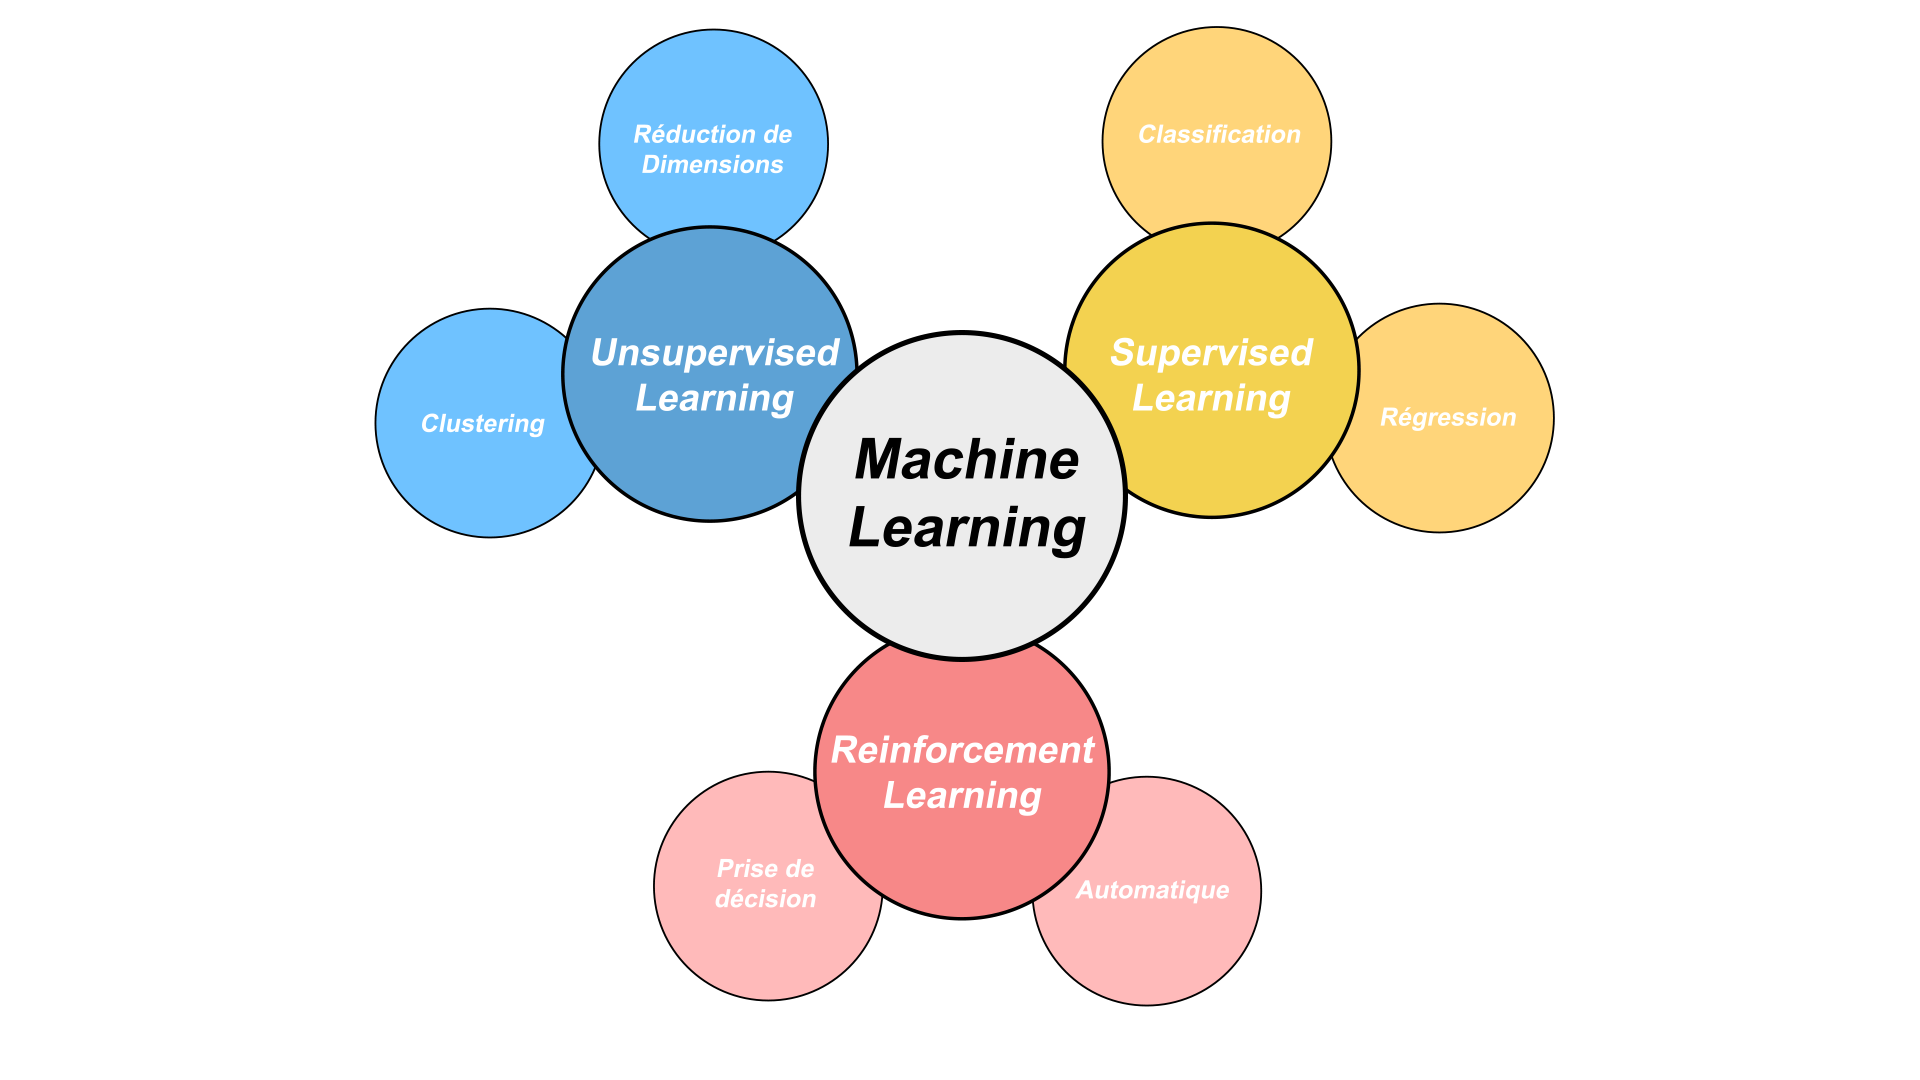
\includegraphics[scale=0.2]{ML_vignette}
	\captionof{figure}{Familles d'algorithmes les plus utilisés}
	\label{fig1}
\end{center}

La première famille, l'appentrissage supervisé (en jaune dans la figure 1.1) consiste à donner des données en entrées, le résultat attendu itéré sur un grand jeu de données afin de trouver la modèle. Pour que le modèle deviennent performant, on fournit un grand volume de données dans le but qu'il se rapproche du modèle attendu.\\

La deuxième famille,l'apprentissage non-surpervisé (en bleu dans la figure 1.1) consiste à apprendre par reconnaitre des ressemblances et des différences entre les données fournies. L'algorithme rassemble les données en groupe suivant ce qui lui semble le plus pertinant. Ainsi quand on passe un modèle bien précis à l'algorithme, il trouve plus facilement car il a été entrainé.\\

Pour finir, il existe une catégorie qui gère sa propre expérience. En effet, l'apprentissage par renforcement (en rouge dans la figure 1.1) consiste à générer ses propres expériences. On se rapproche de l'automobile autonome, la machine change ses états suivant les actions qu'elle entreprend de faire. Un système de récompense positive et négative est mis en place pour constituer une nouvelle expérience et rendre la machine attentive pour maximiser ses chances de réussite.\\
\pagebreak

Pour conclure, le ML est une technologie qui vise à trouver des modèles, comprendre des comportements afin de prédire les besoins d'une application suivant un utilisateur.\\

On peu constater que ce type de besoin se focalise sur une application spécifique cependant, le ML connait des limites au niveau des complexités combinatoire [x: ], or certaines applications nécessitent des applications plus complexes avec plus d'entrées, tels que le traitement des images. Pour palier aux limites du ML, le Deep Learning a vu son essort [x: lien vers essort DL]
\pagebreak



\chapter{Deep Learning}
\section{Le concept du Deep Learning}

Le Deeo Learning est basé sur un système d'un réseau neuronal inspiré des systèmes cérébraux. Ce type d'apprentissage est d'y supervisé car c'est le développeur qui va décidé sur quel type d'apprentissage il va lancer le Deep Learning. Cette technique à besoin d'énormément de données, on parlera donc de Data Lake. 

Pour que le modèle mathématique deviennent performant, il faudra l'entrainer à reconnaitre un élément en particulier. Prenons le cas de la reconnaissance d'un animal. Pour la phase d'apprentissage nous passerons au système plusieurs images d'animaux. On précisera dans la partie d'entrainement les éléments auquels le système devra être conscient.


\pagebreak

\section{L'entraînement du Deep Learning}

Pour notre exemple, les boules vertes représente le bon chemin que le système va prendre pour arriver à vérifier le modèle qui était demandé. Les boules bleus sont celles qui ont des caractéristiques avec le modèle mais ne correspondra pas exactement au modèle qui était demandé. Les boules rouges quand à elles, représentent les erreurs que le système a exclu pour pouvoir apprendre le modèle exacte. Les erreurs sont par la suite renvoyées en amont du système pour que le système ajuste son modèle mathématique

\begin{center}
	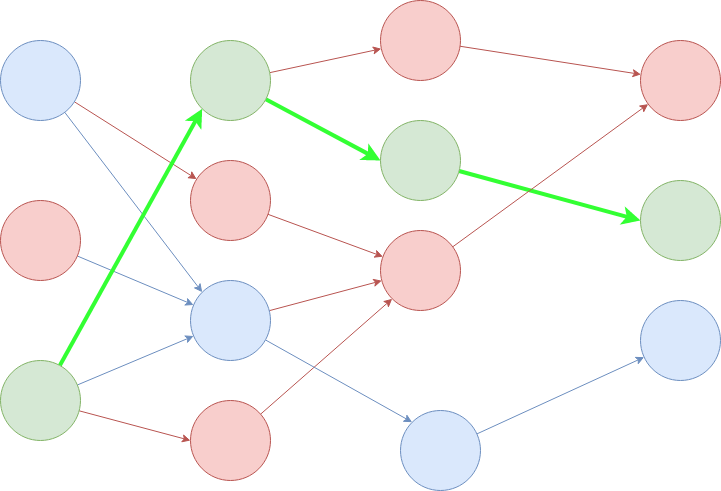
\includegraphics[scale=0.4]{deep_learning_schema}
	\captionof{figure}{Autoapprentissage Deep Learning}
	\label{fig1}
\end{center}

On peut constater que ce type d'algorithme peut être très vite devenir énergivore. De plus, de DL se focalise principalement sur une application. Or, il peut être intéressant d'étudier plusieurs applications similaires afin d'identifier des modèles plus poussés. C'est dans ce contexte que nous allons introduire le Federated Learning.


\chapter{Federate Learning}
\section{Définition du Federate Learning}

En quelques mots, c'est un apprentissage automatique distribué qui permet d'entraîner un modèle mathématique avec un large groupe de données décentralisées qui se trouvent sur des téléphones portables(pour notre cas ici).


\section{Algorithme de Federate Learning}


\section{Implémentation}
Dans notre modèle, nous allons utilisé le système TensorFlow pour former notre système neuronal. TensorFlow est une bibliothèque open source pour le Machine Learning. C'est un petit couteau Suisse qui contient ici des outils pour permettre de résoudre des problèmes mathématiques. 

\section{Deep Learning, cas d'utilisation}

\subsection{Smart Building}

\subsection{Industrie}




\begin{thebibliography}{9}

	\bibitem{lamport94}
	  Leslie Lamport,
	  \emph{\LaTeX: A Document Preparation System}.
	  Addison Wesley, Massachusetts,
	  2nd Edition,
	  1994.
	  
	\bibitem{bigdata}
	Pour la partie sur le Machine Learning https://www.lebigdata.fr/machine-learning-et-big-data

\end{thebibliography}


\label{Pour la partie sur le Machine Learning https://www.lebigdata.fr/machine-learning-et-big-data}

\label{TensorFlow : https://www.lebigdata.fr/tensorflow-definition-tout-savoir}

%Citeseer citeseer.ist.psu.edu,Google Scholar scholar.google.com,ScienceDirect www.sciencedirect.com,ACM Digital Library portal.acm.org,IEEE Digital Library www.computer.org/portal/site/csdl/index.jsp


\label{https://www.youtube.com/watch?v=QR1SnCRungE&ab_channel=AlainOlivetti} 


\begin{appendix}
 \chapter{Annexe}
 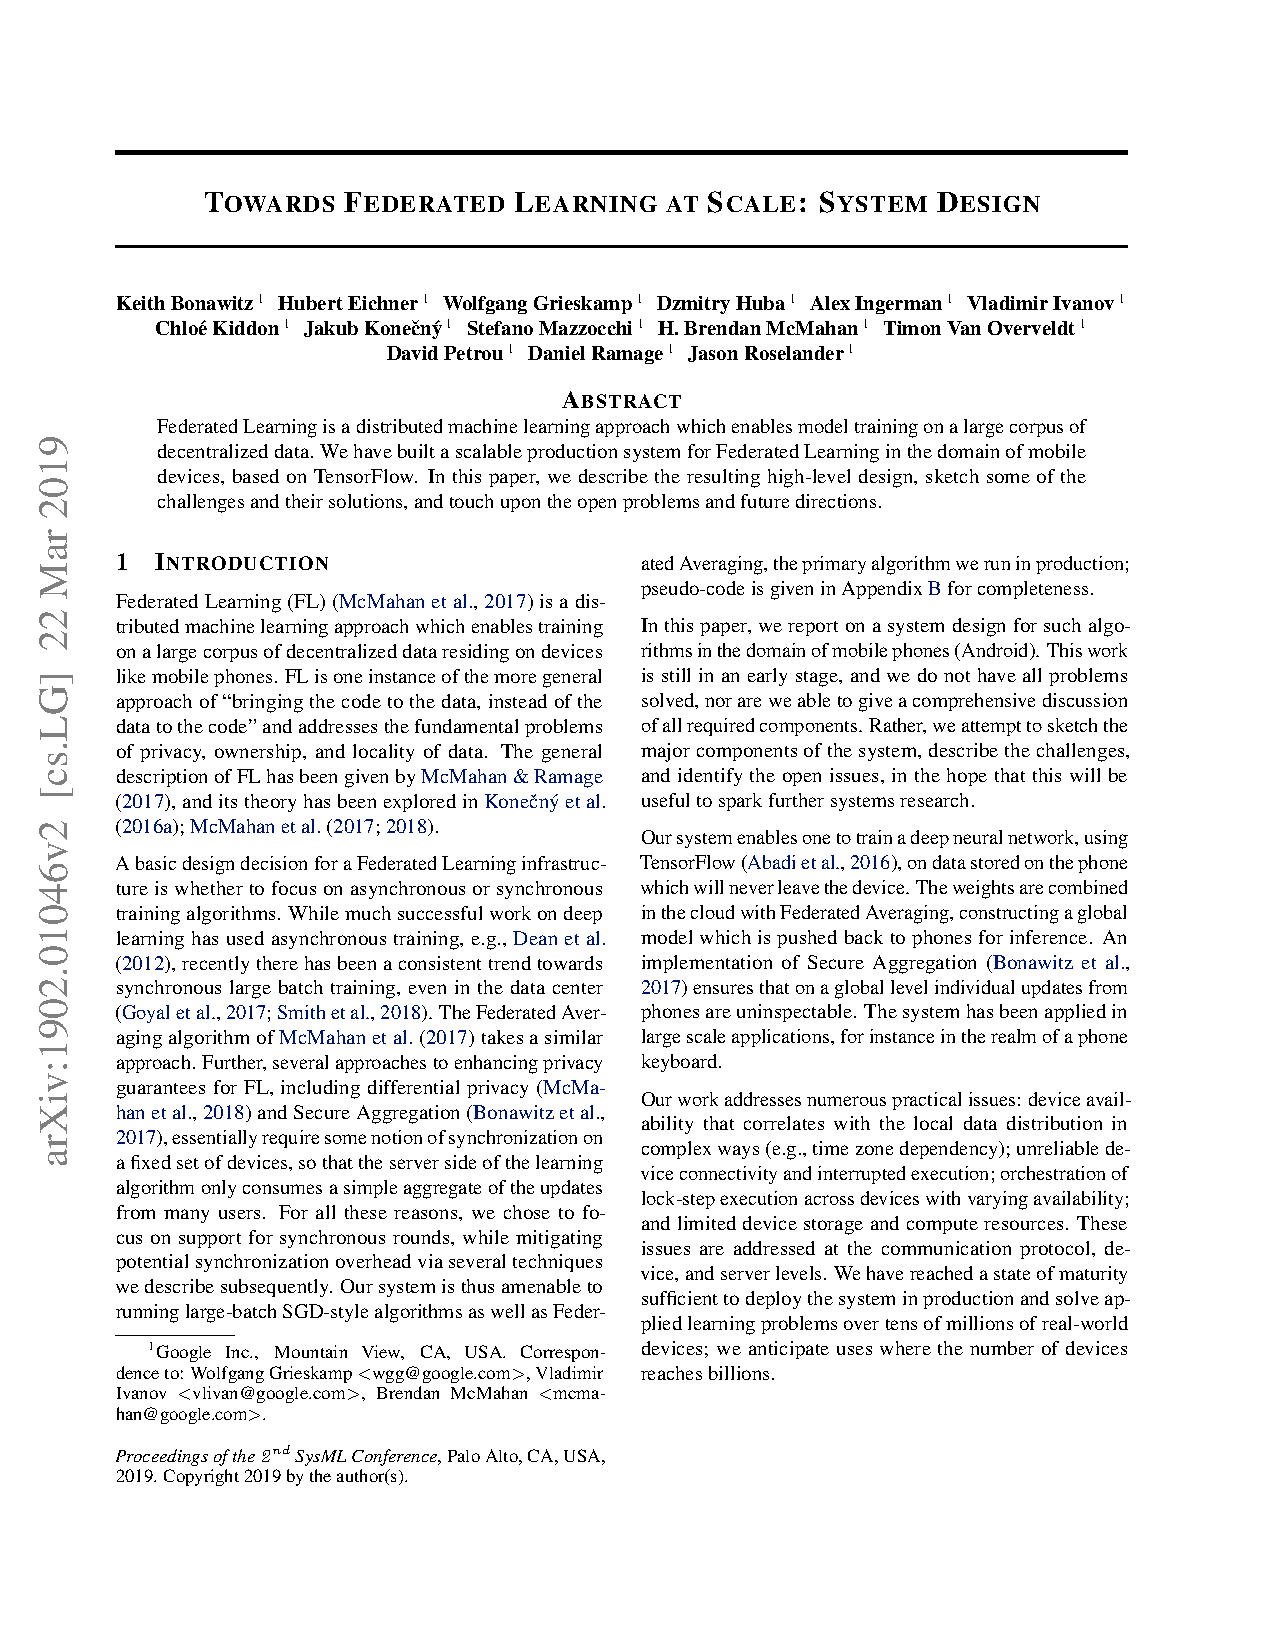
\includepdf{pdf/federate_learning_en.pdf}
\end{appendix}

\end{document}
